\subsubsection{Scopo}
Lo scopo del processo è produrre il \PPdoc , al fine di pianificare e gestire i ruoli che i membri dovranno assumere.
\subsubsection{Aspettative}
Le aspettative del processo sono:
 \begin{itemize}
  \item produrre il \PPdoc ;
  \item definire i ruoli dei membri del gruppo;
  \item definire il piano per l'esecuzione dei compiti programmati.
 \end{itemize}
\subsubsection{Descrizione}
 
\subsubsection{Ruoli di progetto}
 In ogni momento temporale ogni membro deve ricoprire almeno un ruolo e, durante tutta la durata del \gl{progetto}, ricoprire tutti i ruoli almeno una volta. Per ogni membro, le ore di lavoro devono essere il più possibile equamente distribuite. L'assegnazione e la rotazione dei ruoli sono pianificate nel \PPdocRR.
 \paragraph{Responsabile}
 Il \RESP{} è il rappresentante e il punto di riferimento del gruppo, nonché colui che si assume le responsabilità delle scelte del gruppo.
 Le responsabilità assunte sono:
 \begin{itemize}
  \item pianificazione e coordinamento delle attività;
  \item analisi e gestione dei rischi;
  \item gestione delle risorse;
  \item approvazione dei documenti;
  \item approvazione dell'offerta economica;
  \item assicurarsi del rispetto delle \NPdoc{} e che vengano rispettate le pianificazioni nel \PPdoc.
 \end{itemize}
 \paragraph{Amministratore}
 L'\AMM{} è responsabile dell'efficienza dell'ambiente di lavoro, in particolare si occupa di:
 \begin{itemize}
  \item studiare e fornire strumenti che migliorano l'ambiente di lavoro, automatizzando il lavoro ove possibile;
  \item gestire archiviazione, versionamento e configurazione dei documenti e del \gl{software};
  \item garantire la qualità del \gl{prodotto}, fornendo procedure e strumenti di monitoraggio e segnalazione;
  \item eliminare le difficoltà sulla gestione di processi e risorse.
 \end{itemize}
 \paragraph{Analista}
 L'\AN{} deve identificare e comprendere il dominio del problema. \\
 In particolare si occupa di:
 \begin{itemize}
  \item mappare le richieste del cliente in specifiche per il \gl{prodotto};
  \item catalogare e spiegare specifiche comprensibili nell'\ARdoc{} e nello \SFdoc{}.
 \end{itemize}
 \paragraph{Progettista}
 Il \PJ{} ha forti competenze sullo \gl{stack} tecnologico usato. \\
 In particolare deve: 
 \begin{itemize}
  \item indicare le tecnologie più adatte allo sviluppo del \gl{progetto};
  \item descrivere il funzionamento del \gl{sistema} progettandone l'architettura;
  \item produrre una soluzione fattibile in termini di risorse.
 \end{itemize}
 \paragraph{Programmatore}
 Il \PR{} si occupa della codifica, in particolare:
 \begin{itemize}
  \item implementa le soluzioni indicate dal \PJ ;
  \item scrive codice documentato, versionato e mantenibile nel rispetto delle \NPdoc ;
  \item realizza e fornisce gli strumenti per verificare e validare il \gl{prodotto}.
 \end{itemize}
 \paragraph{Verificatore}
 Il \VER , disponendo di una profonda conoscenza delle \NPdoc , si occupa delle attività di \gl{verifica}. \\
 In particolare deve: 
 \begin{itemize}
  \item controllare il rispetto delle \NPdoc durante ogni attività del \gl{progetto}.
 \end{itemize} 
\subsubsection{Comunicazioni}
 \paragraph{Interne}
 È stato creato un gruppo Telegram, accessibile solo ai membri del team, per effettuare le comunicazioni interne. In caso siano necessaria maggiore interazione, si farà utilizzo di \gl{Google Hangouts}. 
 \paragraph{Esterne}
 È stata creata un'apposita cartella di posta elettronica per mantenere i contatti con il \gl{proponente}, il committente ed altre eventuali figure esterne.
 La gestione della casella di posta elettronica è compito del \RESP. \\
 L'indirizzo e-mail è il seguente: \EMAIL.
\subsubsection{Incontri}
 \paragraph{Interni}
 Ogni membro del team può proporre un incontro interno tramite il \gl{bot} Telegram "\gl{VotePoll}", specificando i motivi e l'oggetto dell'incontro. 
 Sarà poi compito del \RESP{} decidere se effettuare l'incontro o meno.\\
  La verbalizzazione degli incontri interni è compito di uno tra gli \AMMP.
 \paragraph{Esterni} 
 Ogni membro del team può proporre un incontro esterno tramite il \gl{Bot} Telegram "\gl{VotePoll}", specificando i motivi e l'oggetto dell'incontro. 
Se il \RESP{} decide che l'incontro può essere organizzato dovrà accordarsi con la figura esterna, e comunicare gli estremi della riunione ai membri del team.\\
 La verbalizzazione degli incontri esterni è compito del \RESP.
\subsubsection{Strumenti di coordinamento}
 \paragraph{\gl{Ticketing}}
 Il \RESP{} ha il compito di assegnare i \gl{task} ai membri del team utilizzando l'applicativo web \gl{Asana}. \\
 Definendo delle \gl{milestone}, è possibile tenere traccia dello stato di avanzamento del lavoro di ogni \gl{task}.
 
\subsubsection{Strumenti di versionamento}
 \paragraph{\gl{Repository}}
 Per il versionamento e l'archiviazione dei file, l'\AMM{} ha creato un \gl{repository} \gl{GitHub}, il quale è disponibile al seguente indirizzo \url{https://github.com/CoCodeSWE}. Tutti i membri del gruppo dovranno creare un proprio account \gl{GitHub}, per poi ricevere i permessi in scrittura sul \gl{repository} da parte dell'\AMM.
 La gestione del \gl{repository} è responsabilità degli \AMMP.
 \paragraph{Struttura del \gl{repository} Docs}
 Al fine di mantenere ordine e coerenza tra i file, il \gl{repository} è così strutturato:
 \begin{itemize}
  \item Docs
   \begin{itemize}
    \item RR
     \begin{itemize}
      \item Esterni: contiene i documenti esterni;
      \item Interni: contiene i documenti interni.
     \end{itemize}
     \item script: contiene gli script utilizzati;
     \item \gl{template}: contiene i \gl{template} utilizzati.
    \end{itemize}
   \end{itemize}
In futuro verranno aggiunte nuove \gl{repository}, le quali strutture saranno rappresentate come precedentemente fatto con Docs.
 \paragraph{Commit}
 Ogni commit effettuata deve essere accompagnata da un messaggio descrittivo delle modifiche effettuate. L'autore della commit dovrà assicurarsi della correttezza dei file. È sconsigliato effettuare il commit di intere cartelle, al fine di evitare inclusioni di file inutili(ad es: file di compilazione).
 Dovrà inoltre essere segnalata l'eventuale aggiunta di nuovi file.
 \subsubsection{Rischi}
 Il \RESP{} ha il dovere di individuare e monitorare i rischi indicati nel \PPdoc. In caso ne vengano identificati di nuovi, il \RESP{} deve agire nel modo seguente:
 \begin{itemize}
  \item comunicare i nuovi rischi al team;
  \item pianificare una strategia per la gestione dei nuovi rischi;
  \item aggiornare le procedure di gestione dei rischi nel \PPdoc.
 \end{itemize}
\subsubsection{Strumenti}
 \paragraph{Telegram}
 Telegram è un \gl{software} libero che fornisce un servizio di messaggistica istantanea erogato senza fini di lucro dalla società Telegram LLC. È stato ritenuto più adatto di Whatsapp.
 \paragraph{\gl{Google Hangouts}}
 Hangouts è un \gl{software} di messaggistica istantanea e di \gl{VoIP}   sviluppato da Google. È disponibile per le piattaforme mobili \gl{Android} e \gl{iOS} e come estensione per il \gl{browser} web Google Chrome. Inoltre, permette la condivisione degli schermi tra i membri della chiamata. È stato ritenuto più adatto di Skype.
 \paragraph{\gl{Git}}
 \gl{Git} è un \gl{software} open-source di controllo versione distribuito utilizzabile dal terminale. Come versione si utilizza la 2.7.4 o superiori.
 \paragraph{\gl{GitHub}}
 \gl{GitHub} è un servizio di hosting per progetti \gl{software}, con il quale è possibile interagire tramite \gl{Git}. \gl{GitHub}
offre diversi piani per \gl{repository} privati sia a pagamento, sia gratuiti, molto utilizzati per lo
sviluppo di progetti open-source. 
\begin{figure}[h]
\centering
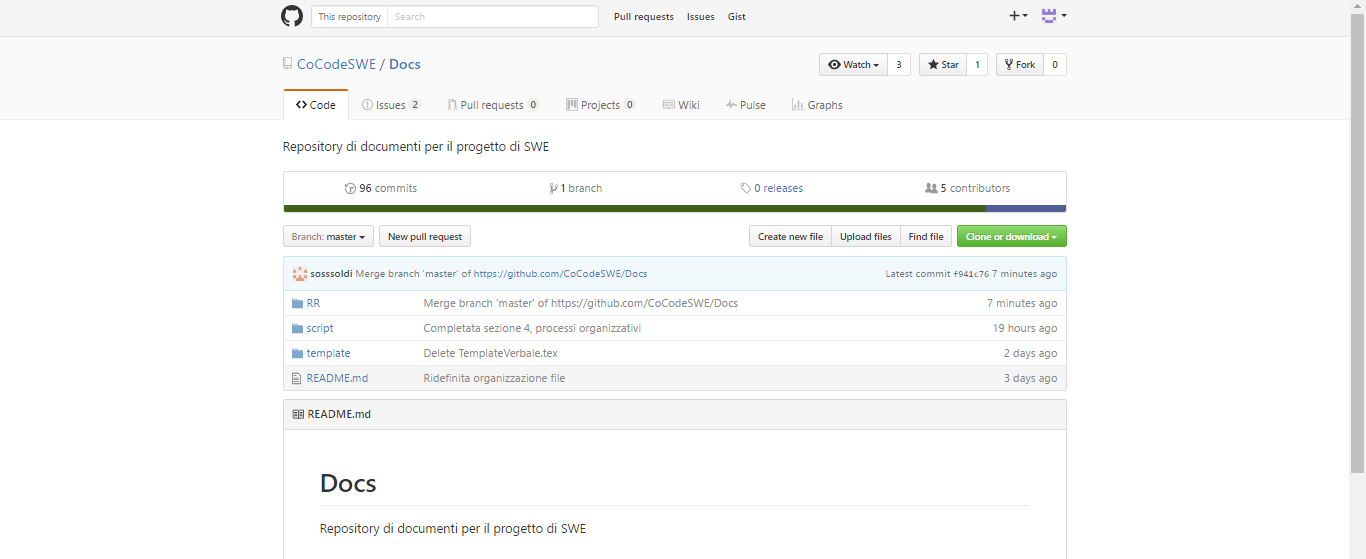
\includegraphics[scale=0.4]{img/github.png}
\caption{Github}\label{sec:Figura4}
\end{figure}
 \paragraph{\gl{GitHub} desktop}
 \gl{GitHub} Desktop è l'applicativo desktop per contribuire e collaborare ai progetti del corrispondente servizio web \gl{GitHub}. Esso è disponibile per Windows e MacOS. Per Windows si utilizza la versione 3.3.3 o superiori.
 \paragraph{\gl{Asana}}
 \gl{Asana} è un applicativo web e mobile che consente al team di assegnare, tracciare e gestire dei \gl{task}.
\begin{figure}[h]
\centering
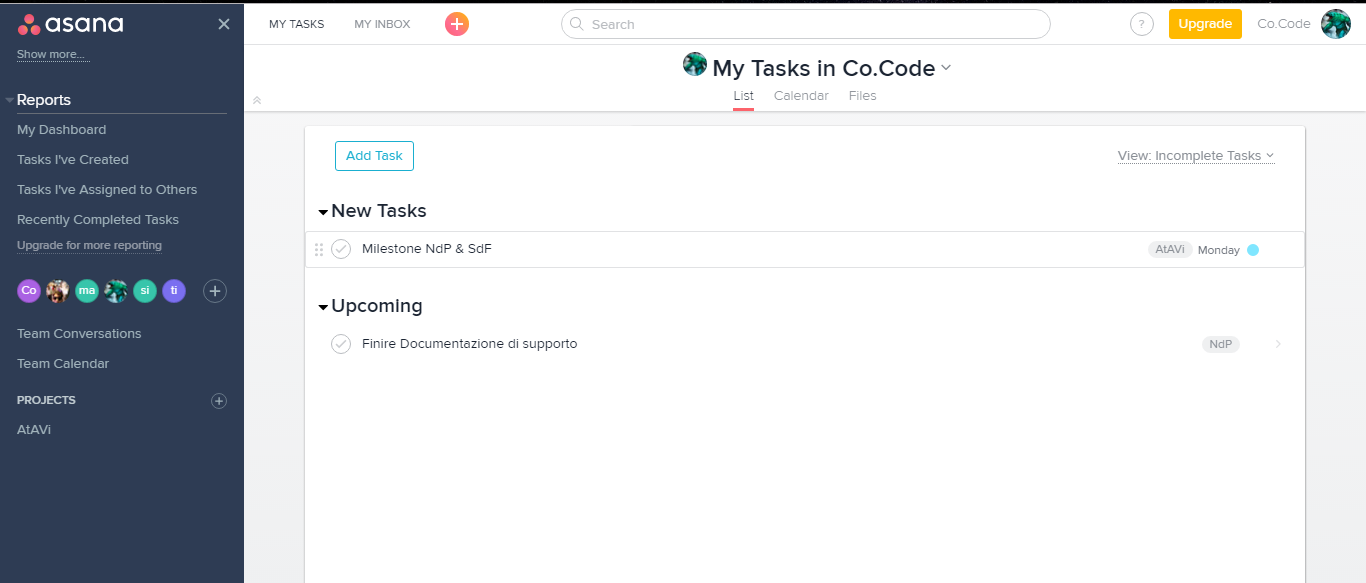
\includegraphics[scale=0.4]{img/asana.png}
\caption{Asana}\label{sec:Figura5}
\end{figure}
 \paragraph{GanttProject} 
 GanttProject è un \gl{software} gratuito per la creazione di grafici rappresentanti l'organizzazione e gestione di compiti e \gl{milestone} all'interno di un \gl{progetto}. Verrà utilizzato nella versione 2.7 o superiore.
\begin{figure}[h]
\centering
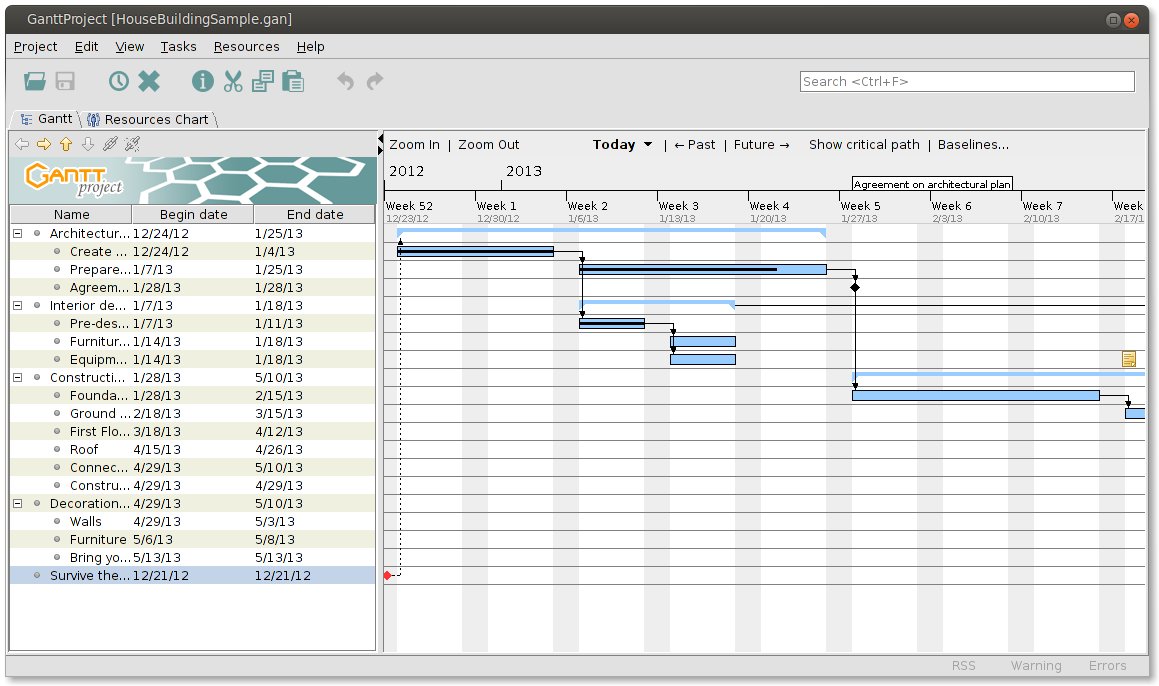
\includegraphics[scale=0.35]{img/gantt.png}
\caption{GanttProject}\label{sec:Figura6}
\end{figure} 
 